%!TEX root = ../thesis.tex

\chapter{Theory}
This chapter describe background theory about parallelism, and why it has become a highly relevant topic in modern system architectures. It also describes the different frameworks and libraries evaluated in this work, as well as some typical parallelizable problems. Finally, benchmarking algorithms are presented and a motivation why each algorithm is suitable for this kind of evaluation.

\section{Background} 
As mentioned in section \ref{sec:IntroductionMotivation}, the performance inclination of single-cored CPU's has reached a limit. The reason for this decline is due to three walls.

The \textbf{ILP-wall} which states that there is not enough instruction level parallelism to keep the CPU busy. Some techniques do however exist such as Very Large Instruction Word (VLIW) and the Superscalar Architecture but are limited by the hardware complexity.

The second wall, the \textbf{Memory wall} is reached because of the gap between the CPU speed and accesses to off-chip memory.

As mentioned in section \ref{sec:IntroductionMotivation} and visualized in figure \ref{fig:CPUstats}, Moore's law is still valid, but the increased amount of on-chip micro transistors needs an increased amount of power, which leads to overheating problems and has been named the \textbf{Power wall}.

The solution to all of these problems are however the same. Although it is not possible to increase the single-thread performance, but we can put more cores on a chip. Today, all major CPU manufacturers develop multi-core CPU's, and most devices used in our everyday life such as smartphones, laptops 
and desktop CPU's have a multi-core architecture, and the number of cores on a chip seems to be increasing, see figure \ref{fig:CPUstats}

\begin{figure}[!h]
    \centering
    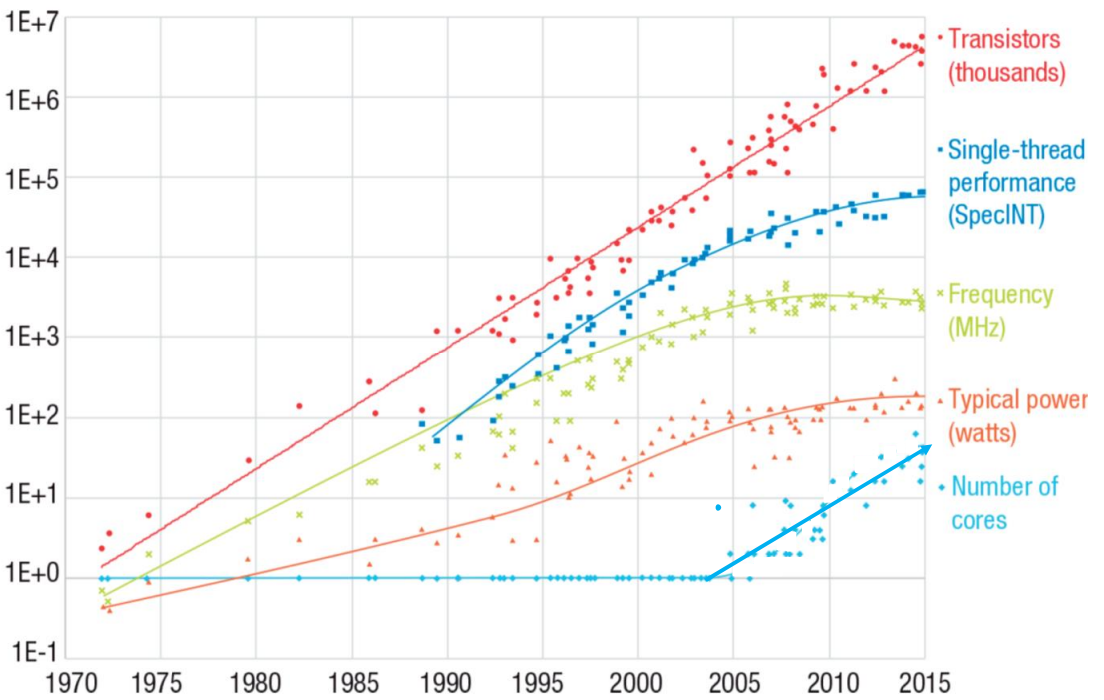
\includegraphics[width=0.8\textwidth]{Introduction/Figs/CPUStats.png}
    \caption{Development of CPU's. \cite{CPUStats}}
    \label{fig:CPUstats}
\end{figure}

The idea of putting multiple cores on a single chip which may be run in parallel is not new technology, GPU's has long been using this architecture and modern GPU chips contains hundreds of cores. This massive amount of parallelism and parallel computing power are designed to render graphics on screen and perform fast algebraic calculations commonly used in computer graphics such as matrix or vector operations, and is thus parallel in nature. But it can also be used for more general purpose computing, as quoted by Thompson et. al. "...Most of this time, however, this power is going unused because it is only
being exploited by graphics applications" \cite{thompson2002gpgpu}.


\subsection{GPGPU History}
With the release of programmable shaders and floating point precision GPU's in 2001, the idea of performing general purpose computing on the GPU became popular. Early research on the subject implemented simple, well-parallelizable problems such as vector or matrix additions, and one of the first scientific GPGPU problems that outperformed the CPU was a implementation of LU factorization. \cite{CUDAtoOpenCL}. Another research on the subject performed by Thompson et. al. from 2002 showed that a simple arithmetic operation applied to all elements of a vector of varying sized, outperformed the CPU once the problem size grew large enough which is generally the case for GPGPU.\cite{thompson2002gpgpu}.

These early adaptations of GPGPU used the traditional rendering pipeline by performing computations in the shaders of the application, using the two major application programming interfaces (API) OpenGL and DirectX. Although this approach adds some limitations, it is still quite widespread and are still in use today. Since then, both OpenGL and DirectX has released shaders specifically purposed for GPGPU. These types of shaders are known as Compute Shaders (CS), and Microsoft released their CS support with the DirectCompute as a part of the DirectX collection of APIs.

Later on Nvidia realized the potential of GPGPU and developed the CUDA framework to make GPGPU programming easier by adding lots of features and simplifying the data transfer. Later on, OpenCL was released with the same purpose, with a lot of backing major companies such as Apple and IBM. It is today maintained by the Khronos group, which also maintains OpenGL.

\section{GPU} \label{sec:GPUTheory}
As previously discussed in section \ref{sec:IntroductionMotivation}, whilst a CPU may have a few cores (~8 cores on a modern desktop machine) that can be run in parallel, modern GPUs have hundreds of cores. Although not as powerful as a single CPU core, this extensive amount of cores allows for massively parallel computation to be made. Moreover, the GPU allows for a much higher theoretical bandwidth than a CPU as is illustrated in figure \ref{fig:GPUGFLOPS}.

\begin{figure}[!htpb]
    \centering
    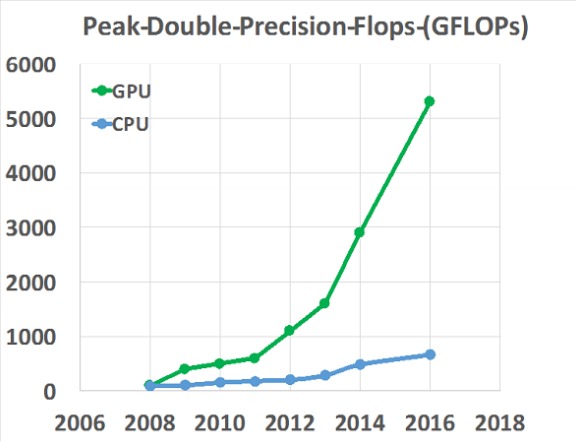
\includegraphics[width=0.6\textwidth]{Theory/Figs/GFLOPSGPU.png}
    \caption{Theoretical giga floating point operations per second (GFLOPS) performance of CPUs versus GPUs. \cite{Ingemar9b}}
    \label{fig:GPUGFLOPS}
\end{figure}
\nomenclature[z-GFLOPS]{GFLOPS}{Giga Floating Point Operations Per Second}

\noindent This is due to the efficient area use of the GPU architecture as visualized in figure \ref{fig:GPUvsCPUArchitecture}, but in particular the SIMD architecture (Single Instruction, Multiple Data). SIMD simplifies the instruction handling since all cores receive the same instruction which is applied to multiple data in parallel, usually stored in list structures such as arrays. The instruction that should be applied to each data-element is often written as a separate piece of code, separated from the main program and run on the device (GPU, FPGA or other parallel hardware). Different frameworks use different languages in which this code is implemented, but the general GPGPU term used for this is a kernel. The most common way of executing a kernel is done in the following steps:
\nomenclature[z-SIMD]{SIMD}{Single Instruction, Multiple Data}
\begin{enumerate}
    \item Allocate memory from the host (typically CPU) to the device.
    \item Copy data from the host to the allocated memory on the device.
    \item Launch the kernel, executing on the data that was just copied.
    \item Copy back the result from the device to the host.
\end{enumerate}

\begin{figure}[!h]
    \centering
    \begin{subfigure}[b]{0.4\textwidth}
        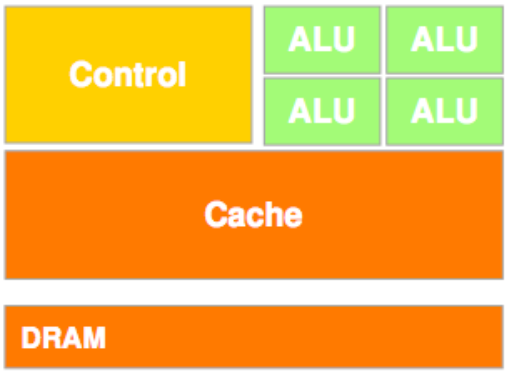
\includegraphics[width=\textwidth]{Theory/Figs/CPUArch.png}
        \caption{}
    \end{subfigure}
    ~ 
    \begin{subfigure}[b]{0.4\textwidth}
        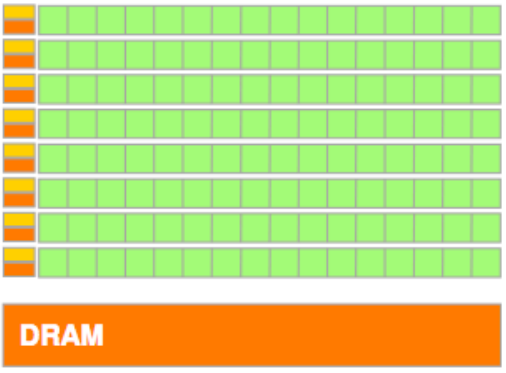
\includegraphics[width=\textwidth]{Theory/Figs/GPUArch.png}
        \caption{}
    \end{subfigure}
    \caption{Area use of CPU (a) and GPU (b)}
    \label{fig:GPUvsCPUArchitecture}
\end{figure}



\section{Frameworks}
This section briefly describes the different frameworks and APIs that are a subject of comparison in this comparative study. Each section contains sample code of a very simple vector addition kernel for the respective frameworks. The popularity of the frameworks is based upon the chart in figure \ref{fig:GoogleTrendsPopularity} from Google Trends.

\subsection{CUDA}
Released in 2007, CUDA developed by Nvidia was the first major GPGPU framework to be released. It aims to make the parallelization of a problem more manageable by providing an easy to work with API. One downside of CUDA is that is has a weak portability and can only be run on Nvidia GPU's. Despite this limitation it is a very popular framework among GPGPU developers, see figure \ref{fig:GoogleTrendsPopularity} \cite{AboutCuda}.  The installation procedure is very simple, all that is needed is a CUDA development toolkit which can be downloaded from Nvidia's webpage.

CUDA is an extension of the C/C++ language, allowing the developer to write both device and host code in a C/C++ like fashion. To run and compile CUDA, a custom compiler is used, NVCC. To define what parts of the code that should be run on the host and the device the keywords \lstinline{__host__} and \lstinline{__device__}, although the \lstinline{__host__} keyword is rarely seen since it is specified per default. To specify that the next block of code is a kernel the keyword \lstinline{__global__} is used.
Each thread in a CUDA program is organized in a block, which in turn is organized in a grid, see figure \ref{fig:CUDAGridBlockThreads}. When launching a kernel, arguments specifying the grid and block-dimension must be supplied. There exists a few different types of memory in CUDA, these memory types are listed in table \ref{tab:CUDAMemoryTypes} 

A very simple CUDA kernel that performs a vector addition can be seen in Listing \ref{lst:cudaVectorAdd}.

\begin{table}

    \begin{tabularx}{\textwidth}{ |X|X|X|X|X| }
      \hline
      \textbf{Memory} &  \textbf{Location} &  \textbf{Cached} &    \textbf{Access} &    \textbf{Scope} \\ \hline 
      \textbf{Register} & On-chip   & Cached    & Access        & Thread \\ \hline 
      \textbf{Local}    & Off-chip  & No        & Read/write    & Thread \\ \hline 
      \textbf{Shared}   & On-chip   & No        & Read/write    & Block \\ \hline 
      \textbf{Global}   & Off-chip  & N/A       & Read/write    & Global + host \\ \hline 
      \textbf{Constant} & Off-chip  & Yes       & Read          & Global + host \\ \hline 
      \textbf{Texture}  & Off-chip  & Yes       & Read          & Global + host \\ \hline 
    \end{tabularx}

\caption{\label{tab:CUDAMemoryTypes} CUDA memory types.}
\end{table}

\begin{figure}[!htpb]
    \centering
    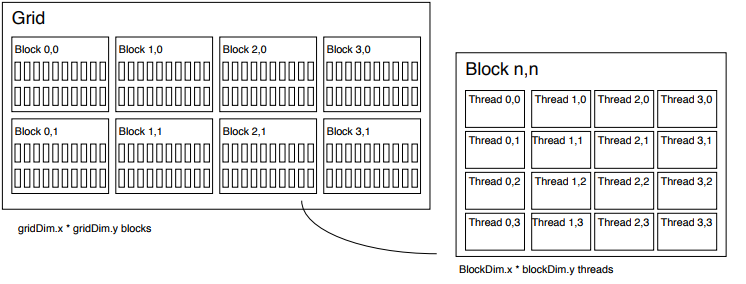
\includegraphics[width=\textwidth]{Theory/Figs/CUDAGridBlockThreads.png}
    \caption{Hierarchical CUDA model for grids, blocks and threads.}
    \label{fig:CUDAGridBlockThreads}
\end{figure}

\begin{lstlisting}[caption={CUDA vector addition kernel}, label={lst:cudaVectorAdd}, frame=single] 
__global__ void add(int *out, const int *in_a, const int *in_b)
{
	int idx = blockDim.x * blockIdx.x + threadIdx.x;
	if (idx < SIZE)
		out[idx] = in_a[idx] + in_b[idx];
}
\end{lstlisting}



\subsection{OpenCL} \label{sec:OpenCLTheory}
For a couple of years, CUDA was the only framework developed for the sole purpose of GPGPU and Nvidia had no competitors on the GPGPU front. That is until Apple took the initiative to develop a competitor, and backed by a lot of major companies, OpenCL was developed. OpenCL sought to offer a more portable and wide variety of parallel devices, and OpenCL offers the ability to run parallel implementations on other devices than just GPU's such as FPGA's and ARM devices. OpenCL is an open standard, and implementations are available from Apple, AMD, Intel, Nvidia and more \cite{KhronosOpenCL}. Because of this, the portability of OpenCL is good, and it can be run on most systems, provided a parallel hardware is present in the system. Since there are multiple implementations of OpenCL, the setup procedure differs, but OpenCL is usually provided by the manufacturers drivers.

The syntax in OpenCL is quite similar to that of CUDA although some differences exist. Although the hierarchy model is very similar, OpenCL uses different terms for these, as well as the memory types. These are listed in table \ref{tab:OpenCLvsCUDA}. Similar to CUDA, OpenCL uses keywords, the keyword that specifies a kernel is \lstinline{__kernel}. Data that resides in the global and local memory are specified using the \lstinline{__global} and \lstinline{__local} keywords.
Whilst CUDA automatically selects a device of the available hardware on the system, OpenCL needs to know what device to run on. Thus the setup procedure differs slightly from the procedure described in section \ref{sec:GPUTheory}. Before copying data and executing the kernel, a OpenCL program first have to do the following steps before doing the steps described in \ref{sec:GPUTheory}:

\begin{enumerate}
    \item Get a list of platforms
    \item Choose a platform
    \item Get a list of devices
    \item Choose a device
    \item Create a context
    \item Load and compile kernel code    
\end{enumerate}

A simple kernel that does the same thing as the CUDA kernel described in listing \ref{lst:cudaVectorAdd}, that is perform a vector addition on two vectors, are given in listing \ref{lst:OpenCLVectorAdd}.

\begin{lstlisting}[caption={OpenCL vector addition kernel}, label={lst:OpenCLVectorAdd}, frame=single] 
__kernel void vectorAddition(__global read_only int* vector1, 
                                __global read_only int* vector2, 
                                __global write_only int* vector3)
{
	int indx = get_global_id(0);
	vector3[indx] = vector1[indx] + vector2[indx];
}
\end{lstlisting}

\begin{table}[!h]
    \begin{tabularx}{\textwidth}{ |X|X| }
      \hline
      \textbf{OpenCL}   &  \textbf{CUDA} \\ \hline 
        Compute Unit    & Multiprocessor (SM)
        Work item       & Thread
        Work group      & Block
        Local memory    & Shared memory
        Private memory  & Registers \\ \hline
    \end{tabularx}
\caption{\label{tab:OpenCLvsCUDA} CUDA vs OpenCL terms}
\end{table}




\subsection{DirectCompute}
Initially released with the DirectX 11 API, DirectCompute is Microsoft's technology for GPGPU, and unlike CUDA or OpenCL which relies on launching kernels, DirectCompute runs a CS as a part of the graphics pipeline. Although released with the DirectX 11 API, DirectCompute runs on GPUs that use either DirectX 10 or 11 \cite{NVidiaDirectCompute}. Since DirectCompute is a part of the DirectX API, no addition additional setup is required, but DirectCompute can only be run on Windows PCs that have a support DirectX version.

Since DirectCompute is not a framework, but a API of the DirectX suite, it is quite different from CUDA or OpenCL. All of the computing in DirectCompute is done on a CS, which would be the equivalent to a kernel in CUDA or OpenCL. The setup process is quite similar to the one described in section \ref{sec:GPUTheory}, but uses the traditional graphics way of copying data between the host and the device, buffers, which are copied to the CS before the CS is run. The CS is written in the high-level shading language (HLSL), developed by Microsoft and a simple CS that performs a vector addition (using a structured buffer) can be seen in listing \ref{lst:DirectComputeVectorAdd}.

\begin{lstlisting}[caption={DirectCompute vector addition CS}, label={lst:DirectComputeVectorAdd}, frame=single] 
struct BufType
{
    int i;
    float f; 
};

StructuredBuffer<BufType> Buffer0 : register(t0);
StructuredBuffer<BufType> Buffer1 : register(t1);
RWStructuredBuffer<BufType> BufferOut : register(u0);

[numthreads(1, 1, 1)]
void CSMain( uint3 DTid : SV_DispatchThreadID )
{
    BufferOut[DTid.x].i = Buffer0[DTid.x].i + Buffer1[DTid.x].i;
    BufferOut[DTid.x].f = Buffer0[DTid.x].f + Buffer1[DTid.x].f;
}

\end{lstlisting}



\subsection{SkePU 2}
SkePU is a high-level skeleton programming framework originally developed by Johan Enmyren and Christoph W. Kessler at Linköping University \cite{enmyren2010skepu}. The framework aims to simplify the parallelization of a implementation by using skeleton functions such as map and reduce which are common parallel algorithms, which makes SkePU very different from the previously mentioned frameworks. When using SkePU, the developer specifies what backend the implementation should run. The currently available backends are sequential C, OpenMP, OpenCL, CUDA, and multi-GPU OpenCL and CUDA \cite{LiUSkePU}. The major revision SkePU 2 was designed by August Ernstsson, Lu Li and Christoph Kessler and is today maintained by August Ernstsson. Further mentions of SkePU will refer to SkePU 2.

Since SkePU is not a GPGPU framework, but a skeleton framework, it is different from the previously discussed CUDA, OpenCL and DirectCompute in terms that it don't involves writing a kernel. Although the setup procedure is quite complicated, once installed it is very portable since it is able to run with most GPU's, depending on the selected backend. As presented in the previous sections, a SkePU vector addition program is supplied in listing \ref{lst:SkePUVectorAdd}

\begin{lstlisting}[caption={SkePU vector addition}, label={lst:SkePUVectorAdd}, frame=single] 

float add(float a, float b){
	return a + b;
}

int main(){
    /**
    ...
    **/
    
    auto addition = skepu2::Map<2>(add);
    
    skepu2::Vector<float> v1(N, 1.0f), v2(N, 2.0f), res(size, 3.0f);
    addition(res, v1, v2);
}



\end{lstlisting}

\begin{figure}[!htbp]
    \centering
    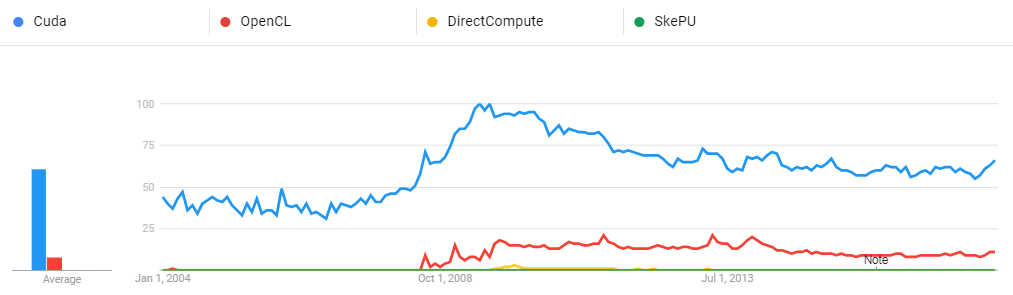
\includegraphics[width=\textwidth]{Theory/Figs/GoogleTrendsComparison.png}
    \caption{Popularity over time of CUDA, OpenCL, DirectCompute and SkePU. Numbers represent search interest relative to the highest point on the chart for the given region and time. \ \textbf{Source:} Google trends}
    \label{fig:GoogleTrendsPopularity}
\end{figure}



\section{Algorithm evaluation}
In this section, algorithms that are suitable for a benchmarking application is briefly explained and discussed. The discussed algorithms are compared, and a motivation of the selected algorithm are given which is explained and discussed further in section \ref{sec:TheoryNBody}.

\subsection{Parallel QuickSort}
A popular sequential algorithm, the QuickSort algorithm invented by C.A.R  Hoare, is a recursive divide-and-conquer based sorting algorithm \cite{hoare1962quicksort}. The algorithm has a time complexity of $O(n \ log \ n)$ in the best case, a worst case complexity of $O(n^2)$, and an average run time of $O(n \ log \ n)$. A pivot element $A[q]$ is selected from the array. The array is then partitioned into two subarrays $A[p...q-1]$ such that all elements are less than $A[q]$, and $A[q+1...r]$ such that all elements are greater than or equal to $A[q]$. After this partitioning step, the pivot are in its correct step. This procedure are then applied recursively to the subarrays until the entire array is sorted. Pseudocode for the algorithm can be seen in Algorithm \ref{alg:quicksort}. The comparison part of the algorithm is well suited for a parallel implementation, but due to the data dependency, parallelizing the partitioning stage is a more difficult task. Some implementations and papers descring how the algorithm can be parallelized do however exist \cite{cederman2009gpu}\cite{sanders1997efficient}\cite{chen2009fast}.

\begin{algorithm}
    \caption{Quicksort pseudocode}
    \label{alg:quicksort}
    \begin{algorithmic}[1]
        \Procedure{quicksort}{$A, lo, hi$}
            \If{$lo < hi$}
                \State $p:=$ \Call{partition}{$A, lo, hi$}
            	\State \Call{$quicksort$}{$A, lo, p-1$}
            	\State \Call{$quicksort$}{$A, p+1, hi$}
            \EndIf
        \EndProcedure
        
        \Procedure{partition}{$A, lo, hi$}
            \State $pivot := A[hi]$
            \State $i := lo - 1$
            \For{$j := lo$ \textbf{to} $hi-1$}
                \If{$A[j] < pivot$}
                    \State $i := i + 1$
                    \State \Call{$swap$}{$A[i],A[j]$}
                \EndIf
            \EndFor
            \If{$A[hi] < A[i + 1]$}
                \State \Call{$swap$}{$A[i + 1],A[hi]$}
            \EndIf
        \EndProcedure
    \end{algorithmic}
\end{algorithm}

A parallel implementation of the Quicksort algorithm would be an interesting algorithm to use for a benchmark application of this degree. The performance of an parallel implementation could be compared to the classical sequential QuickSort algorithm for varying problem sizes, although due of the triviality of the implementation this algorithm was discarded.

\subsection{Distance transform}
First presented by C.Green of Valve Softworks, a method which allows improved rendering of glyphs composed of curved and linear elements was proposed \cite{green2007improved}. The technique works by generating a distance transform (DT) from a high-resolution texture by measuring the distance between a background texel to the closest foreground texture. The distance field is then stored into a channel of a lower-resolution texture, resulting in a texture with a arbitrary resolution, whilst occupying a small amount of video random access memory (VRAM). This low-resolution texture can then be rendered by using alpha-testing and alpha-thresholding features of modern GPU's with great results as illustrated in figure \ref{fig:GreensDT}. 

\begin{figure}[!h]
    \centering
    \begin{subfigure}[b]{0.27\textwidth}
        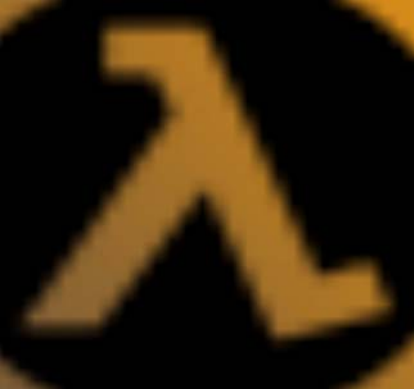
\includegraphics[width=\textwidth]{Theory/Figs/ValveAlphaBlended.png}
        \caption{Alpha-blended}
        \label{fig:valveA}
    \end{subfigure}
    ~
    \begin{subfigure}[b]{0.3\textwidth}
        
\includegraphics[width=\textwidth]{Theory/Figs/ValveAlphaTested.png}
        \caption{Alpha tested}
        \label{fig:valveA}
    \end{subfigure}
    ~ 
    \begin{subfigure}[b]{0.3\textwidth}
        
\includegraphics[width=\textwidth]{Theory/Figs/ValveGreensTechnique.png}
        \caption{Green's technique}
        \label{fig:valveC}
    \end{subfigure}
    \caption{Vector art encoded in a 64x64 texture using (a) simple bilinear filtering (b) alpha testing and (c) Green's distance field technique}
    \label{fig:GreensDT}
\end{figure}

S. Gustavson et. al. later proposed an improved version of Green's technique, using the Euclidean distance to generate a DT \cite{gustavson2011anti}. Whilst Green's description of the proposed algorithm was quite sparse, Gustavson et. al. technique described the general implementation more detailed. Although the general technique described by Green and Gustavson et. al. only describe the two dimensional case, the distance transform has also been extended to three dimensions \cite{jones20063d}. 

One of the problems with the discussed distance transform is the ability to produce sharp features such as corners, and solutions to this problem has not been further investigated. Since the technique works on pixel/voxel level, the algorithm is well parallelizable, and an idea to further investigate this discussed problem was presented. This would however drift apart from the main idea of this research and was thus discarded.

\subsection{N-Body} \label{subsec:TheoryNBody}

The final proposed algorithm is the N-Body problem. Although the base implementation of the algorithm is fairly trivial and embarrassingly parallel, the algorithm can be further optimized by using the Barnes-Hut algorithm, reducing the time complexity from $O(n^2)$ to $O(n \ log \ n)$ \cite{barnes1986hierarchical}.  The N-Body problem as well as the Barnes-Hut algorithm is further described in section \ref{sec:NBodyTheory}.

\subsection{Choice of algorithm}

The choice of algorithm to be implemented and used to evaluate the different frameworks in this work was motivated to be complex enough so that a fair comparison between the frameworks could be made. If the algorithm was to trivial or embarrassingly parallel, the risk would be that framework specific features could be less utilized, and it would be difficult to compare the frameworks in this aspect. It would also raise the risk where the framework-part of the implementation is to small for a fair comparison to be made. 

With this in mind, the algorithm had to be complex enough so that a fair comparison could be made, but not to complex so that the algorithm couldn't be implemented in the given amount of time. Another motivation of the choice of algorithm was that it would include more complex data structures, and not just lists like arrays or vectors. 

The algorithm that best suits this motivation is the N-Body problem when optimized using the Barnes-Hut algorithm. Although the base case of the algorithm is embarrassingly parallel and fairly trivial to implement in any of the discussed frameworks, when optimized using the Barnes-Hut algorithm it gets more complex. The implementation must be able to handle the creation and traversal of trees which is not a very common implementation in GPGPU applications.

\section{N-Body} \label{sec:NBodyTheory}
The following section will describe the theory behind N-Body problem. A description of base problem is presented, followed by a description of the Barnes-Hut algorithm, and how it can be applied to the N-Body simulation to improve the performance.

\subsection{Base problem}
An N-body simulation is a numerical approximation of the behaviour of bodies in a system. A common implementation of the N-Body problem is a astrophysical simulation where each body represents a celestial body such as a star, galaxy or planet. Other astrophysical applications of the N-body problem can be used on a smaller scale to simulate a e.g. 3-body simulation of the earth, moon and sun. The simulation approximates how the celestial bodies behave over time when each body is affected by gravitational forces from all the others. It has also been used in physical cosmology, where N-Body simulations have been used to study the formation of e.g. galaxy filaments and galaxy halos from the influence of dark matter. \cite{navarro1996structure}

The N-body problem has also been used in Plasma physics, where the bodies are ions or electrons, and in molecular dynamics where the bodies represent molecules or atoms (usually in fluid state). In fluid dynamics the vortex blob method for solving Navier-Stokes equations, and boundary value problems have been solved rapidly by using N-Body methods. \cite{greengard1988rapid}

Another application where the N-Body simulation are known to be used is protein folding, where N-body simulations are used to calculate electrostatic and van der
Waals forces. It is also used in the computer graphics field, where it is used for turbulent fluid flow simulation and global illumination computation. \cite{nyland2007fast}.

The simulation made in this work is a astrophysical simulation of a cluster of stars, where each star is affected by gravitational forces from all others. As mentioned earlier this is one of the most common applications of N-Body problem and many papers and implementations regarding this kind of simulation has been made earlier \cite{aarseth2003gravitational}\cite{burtscher2011efficient}\cite{nyland2007fast}. 

\subsubsection{General formulation}
Consider $n$ point masses $m_i$ where $i \in [1, 2,..., n]$. Each point mass has a position vector $p_i$ in two or three dimensional space $\mathbb{R}^3$. 
Newton's second law states that mass times acceleration $m_i \frac{d^2 \boldsymbol p_i}{dt^2}$ is equal to the sum of all of the forces applied on the mass. In a astrophysical simulation, the only force applied to a body is the gravitational force, and Newtons law of gravity says that the gravitational force applied to a mass $m_i$ by a mass $m_j$ is given by the equation
\begin{equation}
    F_{ij} = \frac{G m_i m_j (\boldsymbol p_j - \boldsymbol p_i)}{|| \boldsymbol p_j - \boldsymbol p_i|| ^3}
\end{equation}
\noindent where $G$ is the gravitational constant and $|| \boldsymbol q_i - \boldsymbol q_j||$ is the magnitude of the distance between the masses. Summing over all masses, the total gravitational force $F_i$ applied to mass $m_i$ results in the n-body equations of motion:
 
\begin{equation} \label{eq:totGravForce}
    F_i = m_i\frac{d^2 \boldsymbol p_i}{dt^2} = \sum_{j=1, j\neq i}^n \frac{G m_i m_j (\boldsymbol p_j - \boldsymbol p_i)}{|| \boldsymbol p_j - \boldsymbol p_i|| ^3}
\end{equation}

Equation \ref{eq:totGravForce} has be be applied to each point mass $m_i$ in each timestep of the simulation, and thus have to be compared to all other $n-1$ point masses in the system resulting in a time complexity of $O(n^2)$. Pseudo-code of this \textit{all-pairs} n-body calculation using equation \ref{eq:totGravForce} can be seen in algorithm \ref{alg:allpairspseudocode}. By analyzing equation \ref{eq:totGravForce} and the pseudocode given in \ref{alg:allpairspseudocode}, we can conclude that there are two parts of the algorithm that can be parallelized. Using $p=n$ processors, the outer for-loop in the main procedure can be parallelized, resulting in each particles body-body interaction is calculated by a single process. Once the particles velocities have been updated, the position updating is embarrassingly parallel.

\begin{algorithm}
    \caption{All pars N-body pseudocode}
    \label{alg:allpairspseudocode}
    \begin{algorithmic}[1]

    \Procedure{BodyForce}{$p_i, p_j$}
        \State $F_i := 0$
        \State $Gm_im_j := G *p_i.m * p_j.m$
        \State $dPos := p_i - p_j$
        \State $distance := dist(dPos)$
        \State $magn3 := abs(dist)^3$
        \State $F_i := Gm_im_j * dPos / magn3$
        \State \Return $F_i$
        
    \EndProcedure
    
    \Procedure{main}{}
    
        \Comment{Update velocities}
        \For{$i:=0$ \textbf{to} $n$}
            \State $p_i := particles[i]$
            \State $F_i := {0,0,0}$
            \For{$j:=0, j\neq i$ \textbf{to} $n$}
                \State $p_j := particles[j]$
                \State $F_i := F_i +$ \Call{$BodyForce$}{$p_i, p_j$}
            \EndFor
            \State \textbf{od} % Inner for loop
            \State $p[i].v = p[i].v + dt*F_i$
        \EndFor
        \State \textbf{od} % Outer for loop
        
        \Comment{Update positions}
        \For{$i:=0$ \textbf{to} $n$}
            \State $p_i := particles[i]$
            \State $p_i.pos = p_i.pos + p_i.v * dt$
        \EndFor
        \State \textbf{od}
    \EndProcedure
        
        
    \end{algorithmic}
\end{algorithm}

Although this all-pairs implementation is straightforward and could be implemented effortlessly, with the time complexity $O(n^2)$ it is not very performance efficient. Various methods to improve the performance of the algorithm has been investigated by using hierarchical methods such as fast multipole method (FMM), the Barnes-Hut algorithm and a radiosity method. \cite{singh1995load}\cite{barnes1986hierarchical} 

Both Barnes-Hut, further discussed in section \ref{subsec:BarnesHut}, and the FMM uses a recursive decomposition of the computational domain into a tree structure. The FMM is very similar to the Barnes-Hut method. The main difference between FMM and Barnes-Hut is that while the Barnes-Hut only computes particle-particle, or particle-cell interactions, the FMM also computes interactions between internal cells directly. Due to the FMM method beeing more complex implementation wise, only the Barnes-Hut algorithm is implemented in this work \cite{singh1995load}. The radiosity implementation is mostly used in computer graphics when computing global illumination and is not further discussed here.

\subsection{Barnes-Hut algorithm} \label{subsec:BarnesHut}
Invented by J. Barnes and P. Hut, the Barnes-Hut algorithm is a hierarchical tree based force calculation algorithm with the time complexity $O(n \ log \ n)$ \cite{barnes1986hierarchical}. The algorithm is described in three dimensional space, but is trivially adapted to two dimensional space as needed. 

The algorithm uses a hierarchical tree-structured subdivision of space into cubic cells, each divided into eight subcells whenever more than one particle is found to occupy the same cell. The root of the tree does thus represent the entire spatial space the particles reside in. When calculating the force applied to a single particle, only particles that are close enough under a certain condition, will be accurately force calculated. Particles that are far away from the particle will have a small impact on the resulting force, and can thus be approximated. In Barnes-Hut this is done by calculating each cells center of mass after the tree has been constructed. The tree is then traversed for each particle, if the cell's center of mass is far enough away from the particle, the entire subtree of that cell is approximated by a single "particle" at the cell's center of mass. If however the cell's center of mass is not far enough away from the particle the cell's subtree must be traversed \cite{singh1995load}. 

The tree is built by recursively adding particles into the initially empty root cell, subdividing into eight children when necessary. The resulting tree's internal nodes are space cells, and the leaves of the tree are individual particles. A two dimensional spatial representation as well as the resulting tree can be seen in figure \ref{fig:BarnesHutTree}. Each node in this tree structure has four children and is thus called an quadtree. In three dimensional space, each node will thus have eight children, and this kind of tree-structure is called a octree.
The tree is then reconstructed at every timestep to avoid ambiguity and tangling. For a timestep $t$, the N-Body simulation procedure can be summarized in the following steps, each which can be run in parallel \cite{burtscher2011efficient}:

\begin{enumerate}
    \item Compute bounding box around all bodies
    \item Build hierarchical decomposition by inserting each body into octree
    \item Summarize body information in each internal octree node
    \item Approximately sort the bodies by spatial distance
    \item Compute forces acting on each body with help of octree
    \item Update body positions and velocities
\end{enumerate}


\begin{figure}[!h]
    \centering
    \begin{subfigure}[b]{0.4\textwidth}
        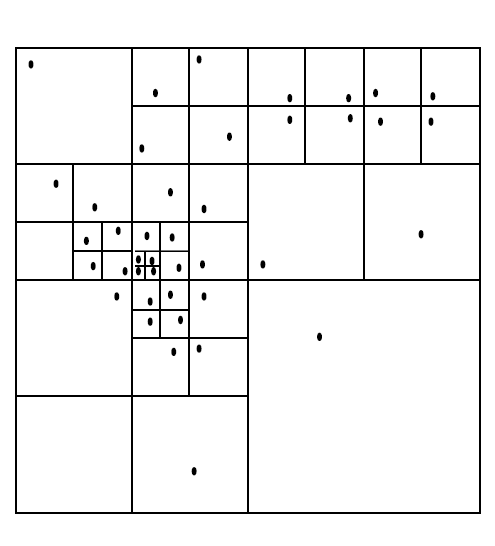
\includegraphics[width=\textwidth]{Theory/Figs/SpatialBarnesHut.png}
        \caption{Spatial domain}
    \end{subfigure}
    ~ 
    \begin{subfigure}[b]{0.4\textwidth}
        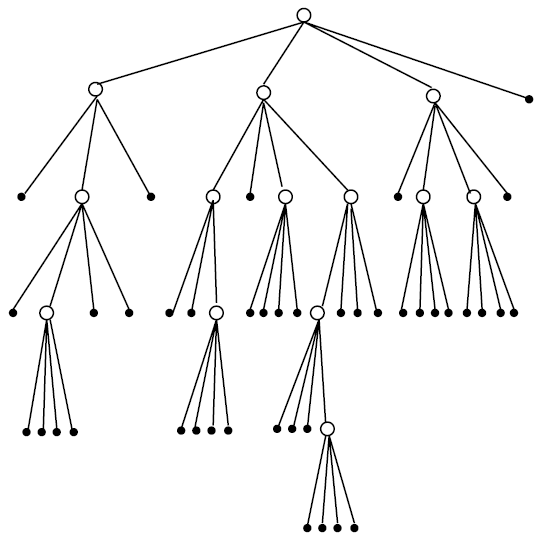
\includegraphics[width=\textwidth]{Theory/Figs/TreelBarnesHut.png}
        \caption{Quadtree representation}
    \end{subfigure}
    \caption{Barnes-Hut recursive subdivision, visualized in 2D for simplicity}
    \label{fig:BarnesHutTree}
\end{figure}


%--------------------------------------------------------%
%----------------------Nomenclature----------------------%
%--------------------------------------------------------%
\nomenclature[z-FMM]{FMM}{Fast Multipole Method}
\nomenclature[z-HLSL]{HLSL}{High-Level Shading Language}
\nomenclature[z-SM]{SM}{Streaming Multiprocessor}
\nomenclature[z-VRAM]{VRAM}{Video Random Access Memory}
\nomenclature[z-DT]{DT}{Distance Transform}
\nomenclature[z-VLIW]{VLIW}{Very Large Instruction Word}
\nomenclature[z-CS]{CS}{Compute Shader}
\nomenclature[z-API]{API}{Application Programming Interface}